\section{Motivation}\label{motivation}

\begin{frame}{Motivation}

\begin{itemize}
\tightlist
\item
  Obtaining feedback from distributed systems can be challenging

  \begin{itemize}
  \tightlist
  \item
    Ongoing assynchronous activities can't stop
  \item
    Processing burden for large systems
  \end{itemize}
\item
  In a resource allocation scenario how to evaluate the fairness of a
  distribution?

  \begin{itemize}
  \tightlist
  \item
    Whose feedback should be trusted?
  \item
    How to deal with divergence on the feedback?
  \end{itemize}
\end{itemize}

\end{frame}

\begin{frame}{Computational Justice Program}

\textbf{Distributive justice}: recent problem in computer systems and
networks (e.g.~operating systems, TCP networks, smart-grids), but
longstanding problem in social relations.

\vspace{0.3cm}

Towards a \textbf{Computational Justice} Framework: social inspired
intelligence applied to technical problems

\begin{block}{}

``Not only must justice be done; it must also be seen to be done''

\end{block}

\end{frame}

\begin{frame}{Problem Statement}

\begin{itemize}
\tightlist
\item
  Network setup:

  \begin{itemize}
  \tightlist
  \item
    \(n\) agents, connected in a graph \(G\), performing independent
    activities and requiring resources to fulfil its tasks
  \end{itemize}
\item
  Availability and demand of resources:

  \begin{itemize}
  \tightlist
  \item
    At a specific time \(t\) (turn), an amount of resources \(P(t)\) is
    made available to all agents and should be shared.
  \item
    Each agent demand \(d_i(t)\) (\(i \in 1, ... ~, n\))
  \item
    \emph{Economy of scarcity}: \(P(t) < \sum_i d_i(t)\)
  \end{itemize}
\item
  Resource allocation:

  \begin{itemize}
  \tightlist
  \item
    Following an allocation policy, agents receive attributions \(r_i\)
    (\(0 \leq r_i(t) \leq d_i(t)\))
  \item
    No leftovers: \(\sum_i r_i(t) = P(t)\)
  \end{itemize}
\end{itemize}

\end{frame}

\begin{frame}{Metrics of Satisfaction}

\begin{itemize}
\tightlist
\item
  Each turn, agents elaborate a metric of \emph{perceived fairness}
  \(\phi_i(t)\), influenced both by \textbf{individual} and
  \textbf{local perceptions} of how resources are being allocated
\item
  The sum of all individual perceptions (\(\Phi(t) = \sum_i \phi_i(t)\))
  becomes a metric for \textbf{general satisfaction}.
\end{itemize}

\begin{block}{}

Given a cluster engaged in repeated rounds of resource distribution and
agents' personal opinions and interactions, how can we ensure that an
allocation is ``fair''?

\end{block}

\end{frame}

\section{Strategy of Solution}\label{strategy-of-solution}

\begin{frame}{Strategy of Solution}

\begin{itemize}
\tightlist
\item
  Use individual subjective assessments

  \begin{itemize}
  \tightlist
  \item
    Decentralisated and independent feedback
  \item
    Convergence of opinions can increase reliability (wisdom of the
    crowds)
  \item
    Gives voice to ``regular'' individuals
  \end{itemize}
\item
  Questions to be considered:

  \begin{itemize}
  \tightlist
  \item
    How to deal with malicious agents, trying to misguide the general
    opinion?
  \item
    How opinions should be weighted, in case of discordance?
  \end{itemize}
\end{itemize}

\end{frame}

\begin{frame}{Strategy of Solution}

\begin{enumerate}
\def\labelenumi{\arabic{enumi}.}
\tightlist
\item
  \textbf{Opinion Formation} - agent opinions are formulated, based on
  individual experience;
\item
  \textbf{Trust} - agents observe their environment and, through
  comparison, define its trusts;
\item
  \textbf{Influence} - agents communicate and diffuse opinions through
  their social influence.
\end{enumerate}

\end{frame}

\begin{frame}{Opinion Formation}

Each individual, in light of the amount of resources received over time
and the amount of resources demanded, can elaborate a personal opinion
of the fairness of an allocation method.

\vspace{0.2cm}

Different possible metrics:

\begin{itemize}
\tightlist
\item
  Average attended demand \[
  \phi_i(t) = \frac{\displaystyle \sum_{s=1}^t 1{\left \{ r_i(s) = d_i(s) \right \}}}{t}
  \]
\item
  Temporal satisfaction \[
  \phi_i(t) =
   \begin{cases}
    (1 - \alpha) \cdot \phi_i(t-1) +  \alpha & \text{if } r_i(t) = d_i(t)\\
    (1 - \beta) \cdot \phi_i(t-1)  & \text{if } r_i(t) < d_i(t)
   \end{cases}
  \]
\end{itemize}

\end{frame}

\begin{frame}{Trust Evaluation}

Having formulated its personal opinion, agents then start to observe
each other opinions, in order to compare their assessments.

\begin{block}{Guiding principles}
\begin{enumerate}
\item \textbf{Affinity}: trust more those who say coherent things (according to yourself!)
\item \textbf{Reinforcement}: It takes time to change an impression
\end{enumerate}
\end{block}

\end{frame}

\begin{frame}{Trust Evaluation}

\begin{enumerate}
\def\labelenumi{\arabic{enumi}.}
\tightlist
\item
  Accordance index \[
  \tau_{ij}(t) = 1 - (1 + \exp^{-k(|\boldsymbol{\bar\phi_{N_i}(t) - \phi_j(t)} | - \epsilon_0)})^{-1}
  \]
\end{enumerate}

where:

\[
\bar\phi_{N_i}(t) = \frac{1}{|N(i)|+1} \sum_{n \in N(i)-\{j\}+\{i\}} \phi_n(t)
\]

\begin{enumerate}
\def\labelenumi{\arabic{enumi}.}
\setcounter{enumi}{1}
\tightlist
\item
  Trust:
\end{enumerate}

\[
T_{ij}(t) = (1 - \gamma) \cdot T_{ij} \left ( t-1 \right ) +  \gamma \cdot \tau_{ij}(t)
\]

(\(T_{ij}(0) = 1\) and \(T_{ij}(t) = 0\) if \(j \not\in N(i)\) )

\end{frame}

\begin{frame}{Influence}

Having the personal opinions \(\phi\) and the trust assessments we can
model the evolution of opinions under social influence.

\[T =
 \begin{bmatrix}
  T'_{11} & T'_{12} & \cdots & T'_{1n} \\
  T'_{21} & T'_{22} & \cdots & T'_{2n} \\
  \vdots  & \vdots  & \ddots & \vdots  \\
  T'_{n1} & T'_{n2} & \cdots & T'_{nn} \\
 \end{bmatrix}; \qquad T'_{ij} = \frac{T_{ij}}{\sum_j T_{ij}}
 \]

\begin{itemize}
\item
  Iterative process of opinion propagation (DeGroot):
  \[\boldsymbol{\phi'(t) = T^{K}\phi} \qquad  (\phi(t) = [\phi_{1}(t), ...~, \phi_{n}(t)]^T)\]
\item
  Final opinion: \[\Phi(t) = \frac{1}{n}\sum_i \phi'_i(t)\]
\end{itemize}

\end{frame}

\begin{frame}{Algorithm summary}

\begin{figure}[htbp]
\centering
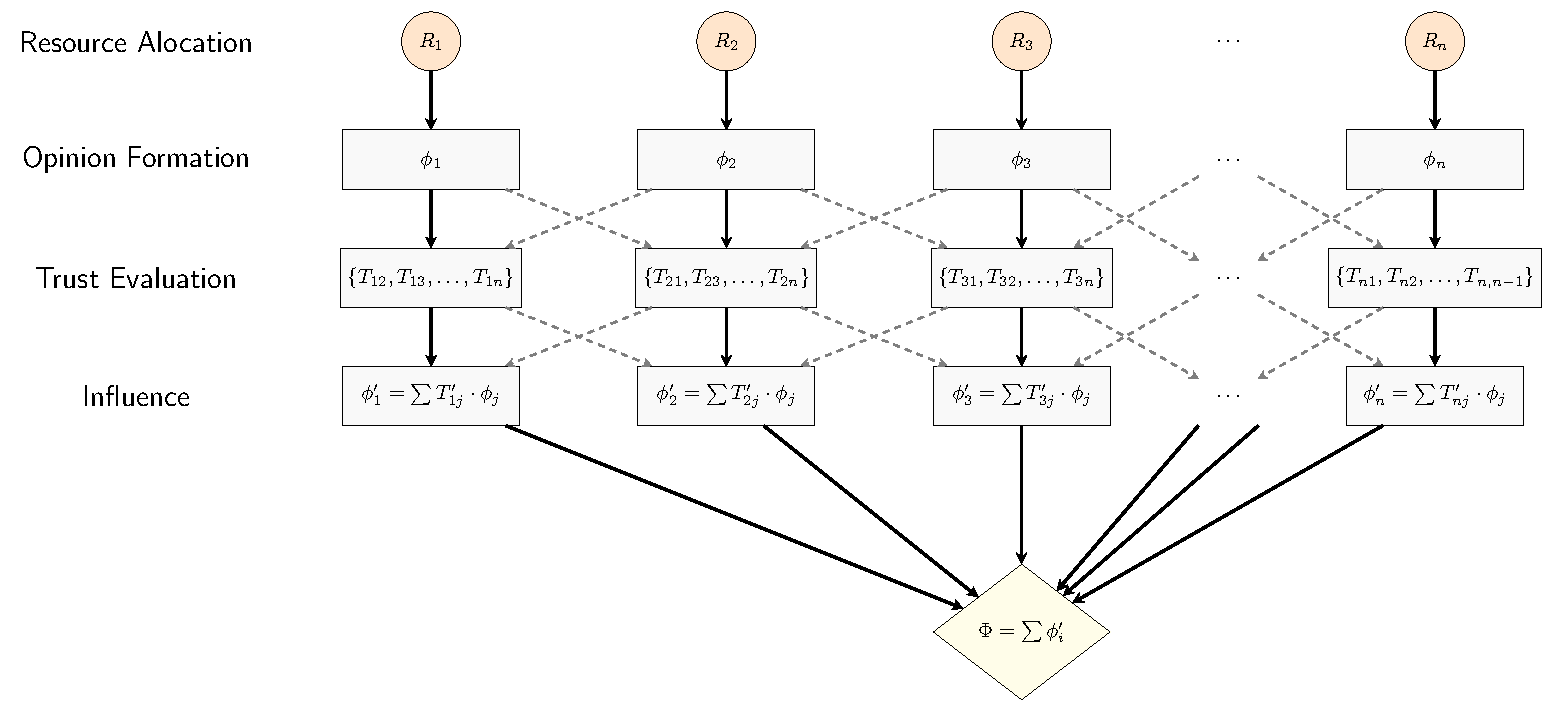
\includegraphics{pics/algdiagram.pdf}
\caption{Complete algorithm}
\end{figure}

\end{frame}

\section{Experiments and Analysis}\label{experiments-and-analysis}

\begin{frame}{Exp 1 - Coherence}

\begin{block}{}
Can the solution identify and distinguish fair and unfair allocation schemes?
\end{block}

\begin{itemize}
\tightlist
\item
  Four allocation methods:

  \begin{itemize}
  \tightlist
  \item
    \emph{Rotation}
  \item
    \emph{Clique first}
  \item
    \emph{Random order}
  \item
    \emph{Ration}
  \end{itemize}
\end{itemize}

\end{frame}

\begin{frame}{Exp 1 - Coherence: Rotation}

\begin{figure}[htbp]
\centering
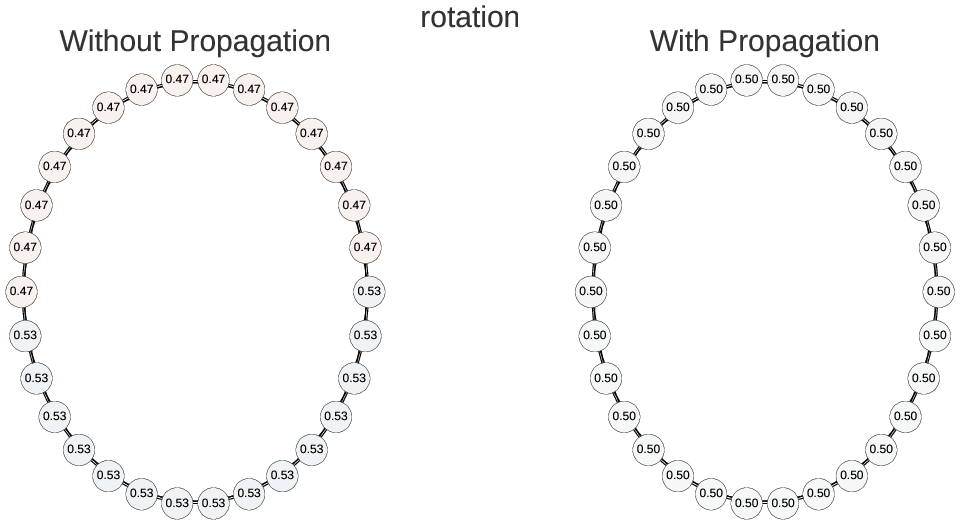
\includegraphics{pics/voices_exp1_rotation.pdf}
\caption{Opinions before and after influence for rotation allocation}
\end{figure}

\end{frame}

\begin{frame}{Exp 1 - Coherence: Clique First}

\begin{figure}[htbp]
\centering
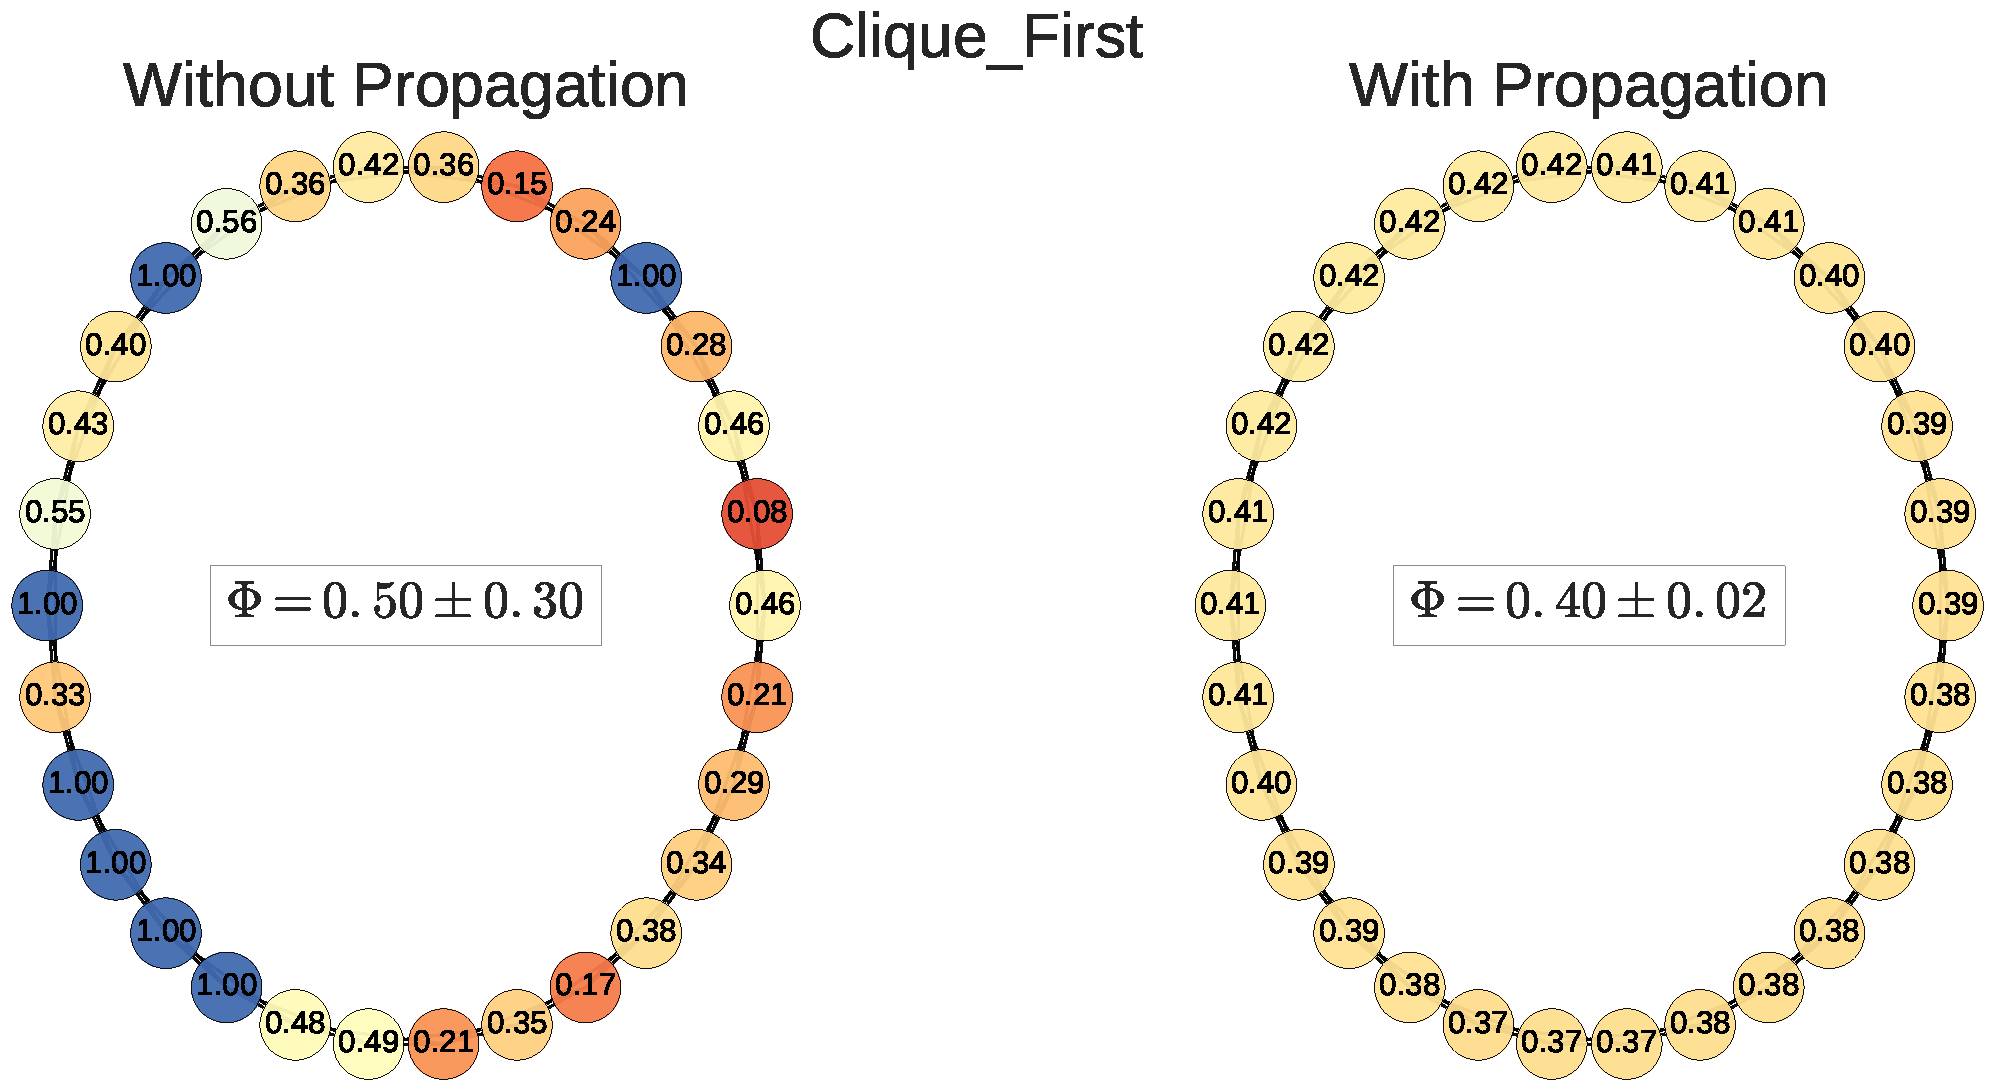
\includegraphics{pics/voices_exp1_clique_first.pdf}
\caption{Opinions before and after influence for clique first
allocation}
\end{figure}

\end{frame}

\begin{frame}{Exp 1 - Coherence: Random Order}

\begin{figure}[htbp]
\centering
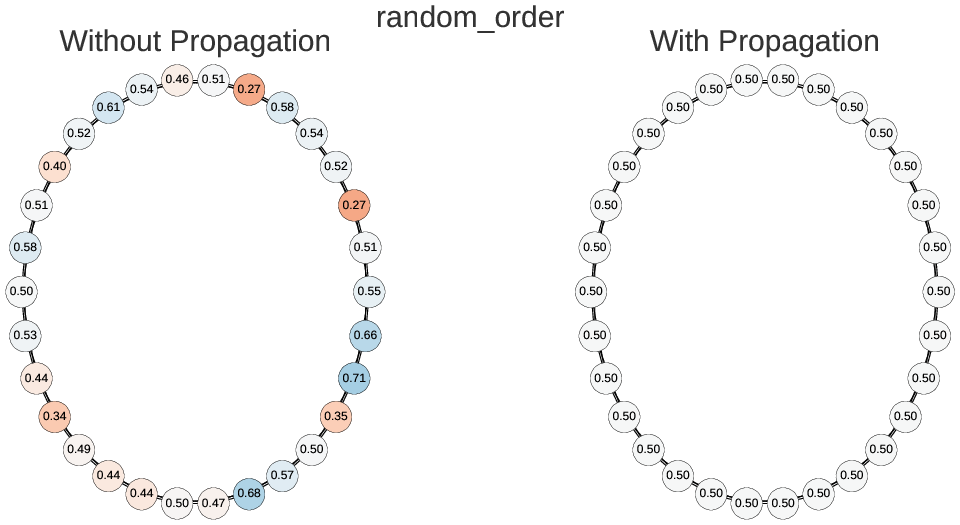
\includegraphics{pics/voices_exp1_random_order.pdf}
\caption{Opinions before and after influence for clique first
allocation}
\end{figure}

\end{frame}

\begin{frame}{Exp 1 - Coherence: Ration}

\begin{figure}[htbp]
\centering
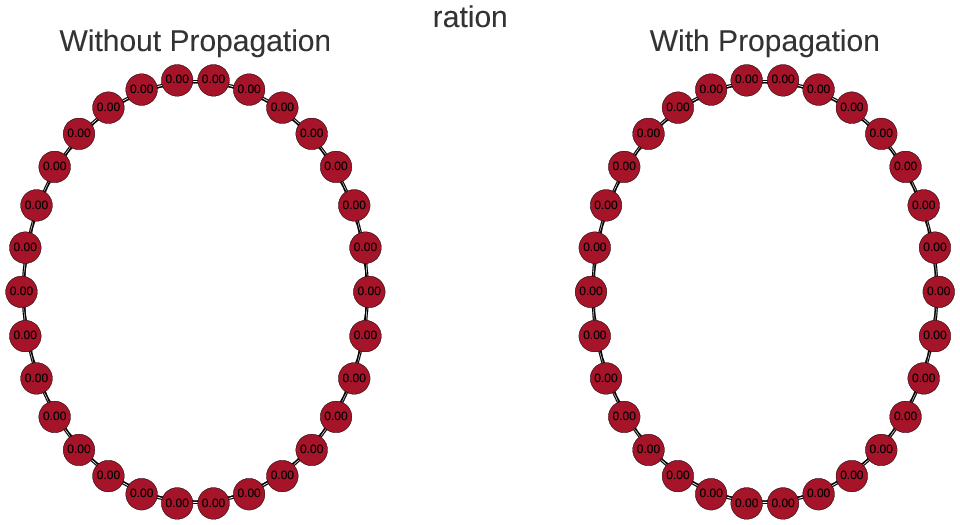
\includegraphics{pics/voices_exp1_ration.pdf}
\caption{Opinions before and after influence for ration allocation}
\end{figure}

\end{frame}

\begin{frame}{Exp 2 - Robustness}

\begin{block}{}
Are there mechanisms able to avoid the influence of malicious agents trying to propagate false information?
\end{block}

\begin{itemize}
\tightlist
\item
  Fair allocation (rotation);
\item
  A group of agents always give negative feedback, regardless their
  situation.
\end{itemize}

\end{frame}

\begin{frame}{Exp 2 - Robustness}

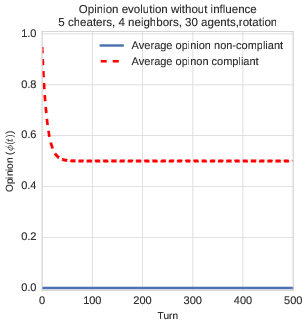
\includegraphics[width=0.45000\textwidth]{pics/voices_rotation_noinfluence_5cheaters_4nei_30agents-opinions.pdf}
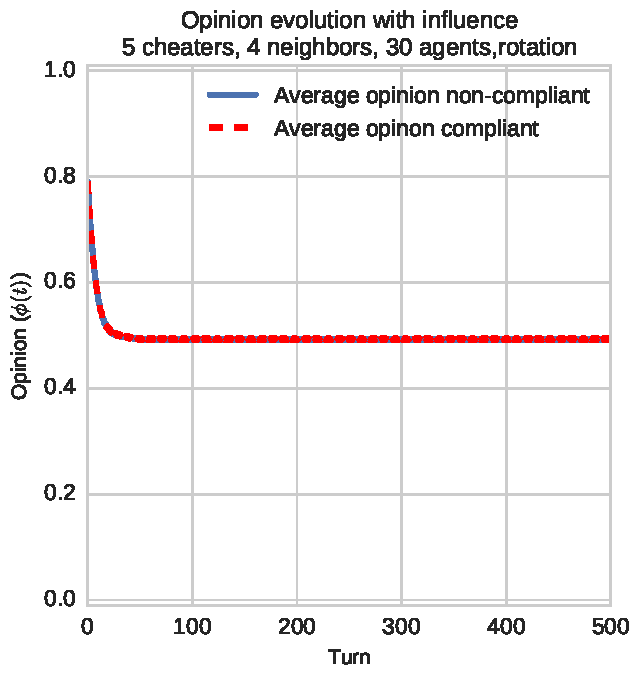
\includegraphics[width=0.45000\textwidth]{pics/voices_rotation_influence_5cheaters_4nei_30agents-opinions.pdf}

\end{frame}

\begin{frame}{Exp 3 - Resilience}

\begin{block}{}
Does it work properly in different topologies and with topology changes?
\end{block}

\begin{itemize}
\tightlist
\item
  Two new topologies tested: small world and random graph 
\item
  In each case, a fair (rotation) and unfair (clique first) allocation
  is tested
\end{itemize}

\end{frame}

\begin{frame}{Exp 3 - Resilience: Small World Network}

\begin{figure}[htbp]
\centering
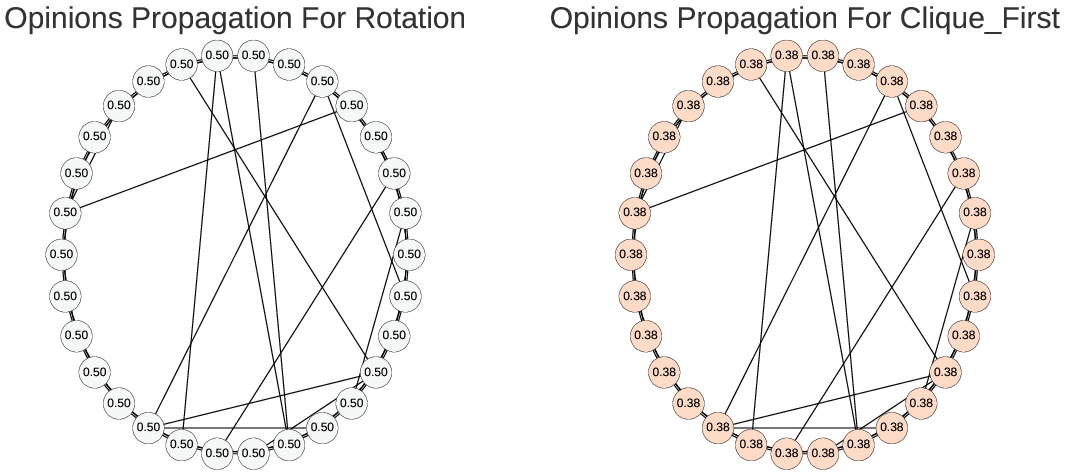
\includegraphics{pics/voices_exp3_small_world.pdf}
\caption{Small World Network}
\end{figure}

\end{frame}

\begin{frame}{Exp 3 - Resilience: Random Network}

\begin{figure}[htbp]
\centering
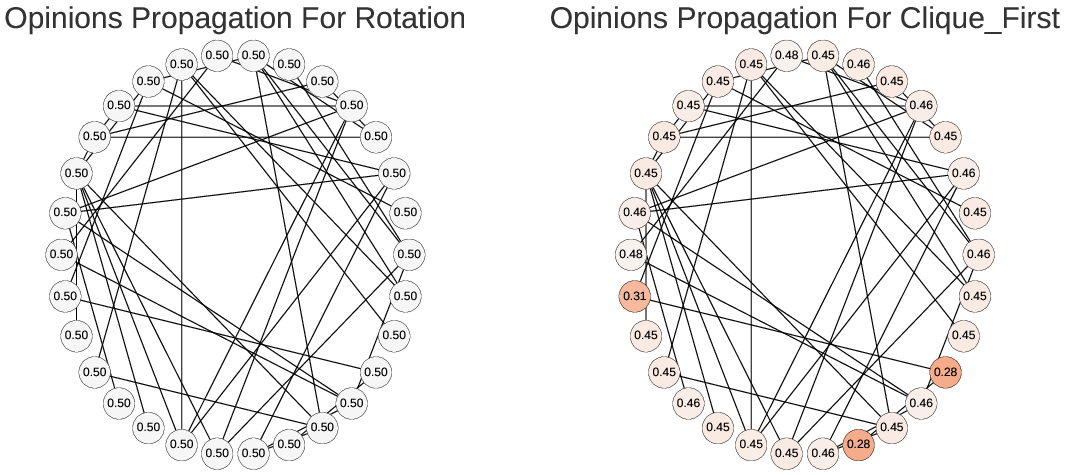
\includegraphics{pics/voices_exp3_random.pdf}
\caption{Random (Erdos Renyi) Network}
\end{figure}

\end{frame}

\section{Conclusion}\label{conclusion}

\begin{frame}{Conclusions}

\begin{itemize}
\tightlist
\item
  Practical method of evaluating the fairness of a resource allocation,
  using subjective assessments, information diffusion and influence
  methods.
\item
  Main features:

  \begin{itemize}
  \tightlist
  \item
    Decentralised and independent computation of the fairness of an
    allocation process;
  \item
    Rapid reaction in case of unfairness -- even when there is initial
    divergence of opinions;
  \item
    Identifying and excluding faulty behaviour (cheating);
  \item
    Robustness to different scenarios and applications.
  \end{itemize}
\end{itemize}

\end{frame}

\begin{frame}{Acknowledgemnts}

\begin{itemize}
\item
  National Council for Scientific and Technological Development (CNPq),
  Brazil;
\item
  Diverse colaborators.
\end{itemize}

\begin{figure}
\centering

\includegraphics[width=0.3\textwidth]{cnpq.png}
\end{figure}

\begin{figure}
\centering

\includegraphics[width=0.3\textwidth]{csf.png}
\end{figure}

\end{frame}
